\documentclass[aspectratio=169]{beamer}

\usepackage{beamerthemesplit}
\usepackage{amsmath}
\usepackage{amsfonts}
\usepackage{amssymb}
\usepackage{cancel}
\usepackage{bussproofs}
%% \usepackage{tkz-graph}

\makeatletter
\newcommand{\reallytiny}{\@setfontsize{\srcsize}{2pt}{2pt}}
\makeatother

\mode<presentation>
{
  \usetheme{AnnArbor}
  \usecolortheme{crane}
}

\usepackage[english]{babel}
\usepackage[latin1]{inputenc}
\usepackage{times}
\usepackage[T1]{fontenc}

\title{Combining learning and reasoning for Bio-AI}

\author{Nil Geisweiller}

\institute[SingularityNET OpenCog Foundations]
{
  \begin{center}
    SingularityNET \& OpenCog Foundations\\
    
\includegraphics[scale=0.32]{images/snet_oc.png}
  \end{center}
}
          
\date[OpenCogCon-20]

\begin{document}

\section{Probabilistic Logic Networks for Bio-AI}

\begin{frame}

  %% I have a small presentation, just to warm us up for an actual
  %% discussion.
  
  \maketitle
\end{frame}

\subsection{Why?}

\begin{frame}
  \frametitle{Why?}

  %% If I ask you what would happen if a bird retracts its wings while
  %% flying in the air, you would immediately answer: it's gonna
  %% fall. But have you ever seen a bird retracting its wings while being
  %% the air. Never. So you see you have an incredibly unbalanced data
  %% here, yet you're able to make an extremely good prediction regarding
  %% an outcome that you've never observed.

  %% And the reason is that you're able to utilize background
  %% knowledge that you have that is relevant to the question, here
  %% the background knowledge is about gravity, which we have an
  %% insane confidence about, and in general beneath the background
  %% knowledge, we can have millions/billions of observations to back
  %% that up.
  
  \center{Why combining machine learning and reasoning?}\\[0.5cm]

  \begin{columns}
    \column{5cm}
    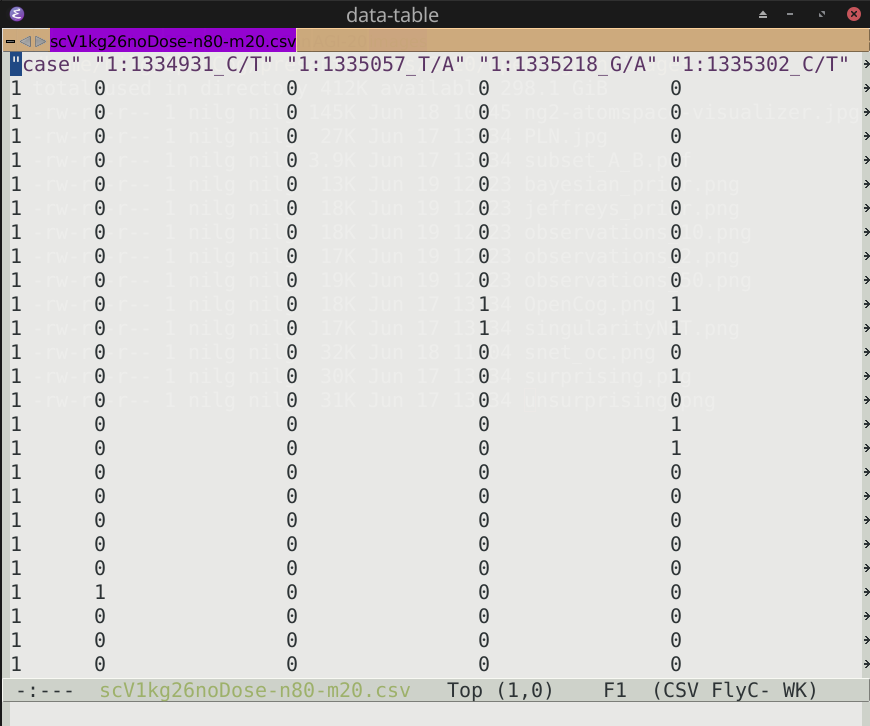
\includegraphics[scale=0.15]{images/table.png}
    \column{0.3cm}
    $\bigotimes$
    \column{5cm}
    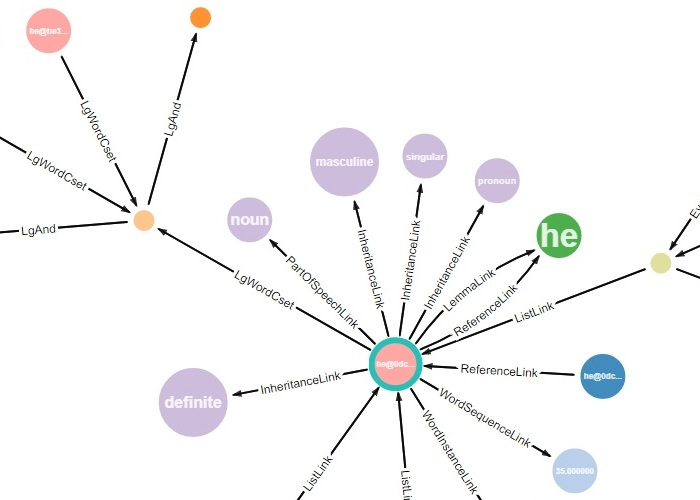
\includegraphics[scale=0.3]{images/atomspace.jpg}
  \end{columns}
  \pause
  \center{%% Background knowledge\\
    %% $\Downarrow$\\
    \alert{Massive amount of indirect evidence}\\[0.2cm]
    \pause
    \textcolor{red}{Ultimate answer to overfitting}
  }
\end{frame}

\begin{frame}
  \frametitle{Why?}

  %% OK, so in this example I'm using the laws of physics as example
  %% of background knowledge, so what about simulation?

  %% And the problem with simulation is that unless it is fairly
  %% constrained or at the precisely the right scale, etc, it's
  %% basically intractable. Simulation in general can only be done if
  %% we short-cut the calculations, using abstractions. An example of
  %% that would be statistical physics, and its works nice, at this
  %% level. But when we want to go to the levels up, biology, etc,
  %% then it no longer works, and what we actually need are mechanisms
  %% that can creates these abstractions.  And for that we need
  %% reasoning (and learning as well, although one can see learning as
  %% a specialized form reasoning).

  \center{What about simulation?}\\[1cm]

  \center{\alert{Impractical without abstractions}\\[1cm]
    %% $\Downarrow$\\[0.5cm]
    \textcolor{red}{Reasoning\\$\Downarrow$\\Abstractions}
  }

\end{frame}

\begin{frame}
  \frametitle{Why?}

  %% And another reason we want to combine reasoning and machine
  %% learning is for meta-learning in general, such as for instance
  %% speeding up learning, but that's a long topic for another time.

  \center{\alert{Help learning (and reasoning)}}\\[1cm]
  
  \begin{itemize}
  \item \color{red}{Reasoning for meta-learning}
    \begin{itemize}
    \item Filtering relevant features
    \item Guide optimization
    \end{itemize}
  \item \color{red}{Learning for meta-reasoning}
    \begin{itemize}
    \item Discover inference control patterns
    \item Create contextual Hebbian links
    \end{itemize}
  \end{itemize}

\end{frame}

\section{Learning \& reasoning over the Bio-AtomSpace}

\begin{frame}
  \frametitle{Learning \& reasoning over the Bio-AtomSpace}

  \begin{itemize}
  \item Learning:\\
    \begin{itemize}
    \item MOSES (program evolution)\\
      $\Rightarrow$ \alert{Predictive models}
    \item Pattern Miner (frequent pattern mining)\\
      $\Rightarrow$ \alert{Discover abstractions}
    \end{itemize}
  \item Reasoning:\\
    \begin{itemize}
    \item Pattern Miner
    \item PLN (Probabilistic Logic Networks)\\
      $\Rightarrow$ \alert{Use existing and discovered background knowledge}
    \end{itemize}
  \end{itemize}
  
\end{frame}

\subsection{Example}

\begin{frame}
  \frametitle{Example}

  Example of reasoning involving MOSES model + discovered pattern +
  background knowledge.
\end{frame}

\subsection{Status and remaining work}

\begin{frame}
  \frametitle{Status}

  \begin{itemize}
  \item Discovered simple patterns
    \begin{itemize}
    \item Pattern size: 2 conjuncts
    \item GO + SMP dataset: 1M atoms
    \item Time: couple hours
    \end{itemize}
  \item Inferred short trails
    \begin{itemize}
    \item Trail size: about 8 steps
    \item GO dataset: 650K atoms
    \item Time: couple hours
    \end{itemize}
  \item Focused on longevity
  \end{itemize}
\end{frame}

\begin{frame}
  \frametitle{Difficulties}

  \begin{itemize}
  \item Porting data into the atomspace
  \item Finding good queries
  \item Very resource hungry (millions of atoms)\\
    \begin{itemize}
    \item CPU: 1 single step can take 20+ minutes
    \item RAM: 1 single step can take 64GB+
    \item Need ECAN!
    \end{itemize}
  \item Advanced forms of reasoning\\
    \begin{itemize}
    \item Stress-test on PLN
    \end{itemize}
  \end{itemize}
\end{frame}

\begin{frame}
  \frametitle{To do}

  \begin{itemize}
  \item Experiment with other domains, COVID-19, Cancer
  \item Complete Multi-threaded Rule Engine
  \item Integrate ECAN
  \item Integrate spatio-temporal reasoning
  \item Experiment with inference control meta-learning
  \end{itemize}
\end{frame}

\end{document}
